%%%%%%%%%%%%%%%%%%%%
%%%%%%%%%%%%%%%%%%%%
%%
%% Andrea Tino - 2019
%% Programming + Science
%% Opinion model
%%
%%%%%%%%%%%%%%%%%%%%
%%%%%%%%%%%%%%%%%%%%

\section{Developing a CA to describe people's opinion change}
\label{sec:opinionca}

In section \ref{sec:simpleca}, we have built our first automaton: Conway's Game of Life.
That CA is a great start because it has many interesting configurations and evolutions;
however, now, we want to move forward and develop another, different, automaton.
A CA is a mathematical model; other than being a very fun thing to play with, it is a
tool that can be used to study our reality from a theoretical perspective. Like any other
model, it is capable of simplifying our universe so that we can study specific things
about a natural phenomenon. CGL was just an automaton we built without a specific goal
in mind, we just wanted to play with automata.
For the next stage, we want to build a CA that can help us reach a distinct objective:
illustrating opinion change among the members of a society.

\subsection{Working out the model}
We want to use a scientific approach to solve a problem. So, 
before going straight to coding, we need to:

\begin{enumerate}
\item Decide what natural phenomenon we want to describe and control. 
We basically want to answer the question: what is the problem we want to solve?
\item Define the mathematical model to reach that objective. We 
basically need to translate
our problem into mathematical terms. This step is called: \textit{modelization}.
\item Create a computer simulation by translating into code the mathematical
model we created, this stage is called: \textit{simulation}. While simulating,
it is possible to collect all sorts of data and measurements; those will be used
to rate which model best achieves the objectives with highest performance and
lowest cost.
\item After all simulations have been run, the best model is selected and then
effectively put in practice. Most of the times, it results in something being
physically built, or a process being enforced. This stage is called:
\textit{implementation}.
\end{enumerate}

% Figure
%
\begin{figure}[b]
\centering
\sidecaption
% tikz diagram
%
% Tikz Diagram
%

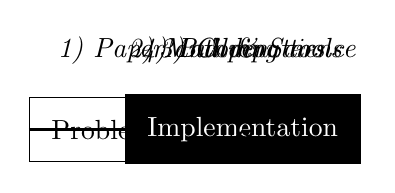
\begin{tikzpicture}

%\pgfdeclareimage{bulb}{assets/light-bulb}

\tikzmath{
	\x = 3.4;
    \sx = \x + \x;
    \ssx = \sx + \x;
    \y = -0.75;
}

\node[draw,inner sep=8pt] (prob) at (0,0) {Problem definition};
\node[draw,inner sep=8pt,fill=gray,text=white] (mod) at (\x,0) {Modelization};
\node[draw,inner sep=8pt,fill=black,text=white] (sim) at (\sx,0) {Simulation};
\node[draw,inner sep=8pt,fill=black,text=white] (impl) at (\ssx,0) {Implementation};

\draw[->,draw=black,thick] (prob) to (mod);
\draw[->,draw=black,thick] (mod) to (sim);
\draw[->,draw=black,thick] (sim) to (impl);

%\node {\pgfbox[center,bottom]{\pgfuseimage{bulb}}};

\node at (0, \y) {\textit{1) Paper and pen}};
\node at (\x, \y) {\textit{2) Math \& Science}};
\node at (\sx, \y) {\textit{3) Computers}};
\node at (\ssx, \y) {\textit{4) Building tools}};

\end{tikzpicture}

%
% If not, use
%\picplace{5cm}{2cm} % Give the correct figure height and width in cm
%
\caption{Illustration of the different phases in the scientific approach to solve a problem.
Each one of them is executed with different tools and require different skills.}
\label{fig:sciappr}
\end{figure}
%

This way of doing things (visualized in figure \ref{fig:sciappr})
is called: \textit{scientific approach} and is at the very core
of what scientists, mathematicians and engineers do every day. So let's start
with the first step: what problem do we want to solve?

\begin{proposition}[Problem definition]
\label{prop:opinionproblem}
Consider the community of people inside a city. The city council has set a goal to reduce
the amount of cars, plastic and pollution on the whole urban area with the intention of
promoting sustainability, green resources, and renewable energies.

The city administration, however, does not have much money to enforce the new green policies
it wants, so it has to rely on the citizens to try to adopt a more green and sustainable life
in complete autonomy. So they have hired us, a group of scientists, to find a solution to
this problem.
\end{proposition}

Proposition \ref{prop:opinionproblem} seems quite tough right? We are now scientists and we
have been given the job to try to convince the inhabitants of a whole town to change their
daily lives and habits to be more green and sustainable (using less plastic, riding bikes instead of
cars, trash fewer objects, etc.). How are we going to do that?
For starters, no panic! We have an approach to follow, so let's use the method pictured in figure
\ref{fig:sciappr} to solve our problem.\\

Where are we in that diagram? We have passed the first stage as we now know what problem we must focus
on. So now it is time to think about the solution and we do that by using Mathematics and Science. What we
want to study is basically a population made of different individuals: men, women and children.
The city council wants us to find a way to persuade the citizens to change their lifestyle. Changing
a person's behavior or habits means to change their opinion on specific matters. No, we are not talking
about \textit{Inception}\footnote{A sci-fi/thriller movie released in 2010 where a group
of people attempt to plant an idea inside a man's mind by violating his dreams. 
If you haven't see
it, you should because it's pretty cool: \url{https://www.imdb.com/title/tt1375666/}.}, we want to
use less drastic/invasive (and more legal) strategies. One common way of doing this is by
running an \textit{advertising campaign} with tv spots and street cartboards to promote
the concepts we want. However remember that we don't have mush money, so we cannot run these ads all
over town as it would be too expensive: we have a limited budget, which means we can only run small
local campaigns in blocks or areas of the city. Would this strategy suffice?\\

From different social studies, like mentioned by Flache et al. \cite{flache-opinion},
it has emerged that people change their opinion also in relation to
the community where they live. Try to think about one time where your opinion about something shifted,
and try to recall what caused that change: most likely it was because you met and talked with another
person about that subject and the conversation made you change your mind. All that being said,
of course folks' opinion doesn't vary so quickly with just one interaction, it depends
on which person we meet and what topic we are focusing on. Also, people are very different: some
change opinion quite easily, while others are much more stubborn.

However, here's the most important point, no matter how easily a person's opinion change, what matters
is that it can actually change and the change is caused by the opinions of other individuals. Is like
if opinions were contagious to a certain extent. So, since we cannot run a town-wide ad campaign, we can
rather do the same but in a few areas of the city to change a few people's mind
about sustainable lifestyle so that they will later influence their neighbors. But how many citizens
do we need to convince to have enough of them so that their influence will spread across the whole town?
Should we run a bigger campaign on a single city block? Or smaller campaigns in more different areas
of town? Or some other strategy?
To answer that question, we are going to use... you guessed it: a CA!\\

To use a CA for our problem, we need to create one, so we must define its properties:

\begin{enumerate}
\item \textbf{What do the cells represent?} A cell represents a single individual (citizen) in the city.
A cell's neighborhood represents the people that live close to that person
(same building, same city block, etc.).
\item \textbf{What is the state of a cell?} Every individual (cell) can be either: \textit{convinced}
($1$, active, black), or \textit{unconvinced} ($0$, inactive, white) about sustainable lifestyle.
\item \textbf{How do we define the state transition function?} The main idea is that a non convinced citizen
would become convinced if there is a sufficient number of his neighbors that are convinced as well.
Of course the opposite applies as well: if a great number of his neighbors is not convinced,
a convinced individual will also turn unconvinced.
\end{enumerate}

We have the basics of our CA, but we need to work more on the transition function. If we read again the
last point in our list above, we can express with simple mathematical expressions what we wrote:

\begin{proposition}[Opinion shift CA transition function]
\label{prop:opicatrans}
Given a cell $y_{i,j} \in E$ in our opinion analysis CA, its next state is defined by this
transition function:
\begin{equation}
f(n) =
  \begin{cases}
    0       & \quad n < N^\ast\\
    1       & \quad n \geq N^\ast\\
  \end{cases}
\end{equation}
Where $n = 0 \dots 8$ is the number of active neighbors of $y$, and $N^\ast = 0 \dots 9$ is a threshold
value.
\end{proposition}

As you can see from proposition \ref{prop:opicatrans}, transition function $f$ uses a value $N^\ast$ to
set a point where a citizen changes his mind, this number is quite important:

\begin{definition}[Turning Point]
\label{def:tp}
When the transition function $f$ is defined as in proposition \ref{prop:opicatrans}, then quantity
$N^\ast$ is called: \textit{Turning Point} (TP).
If at least $N^\ast$ neighbors are convinced about
a topic, then a citizen would turn or remain convinced too, while if the number of convinced neighbors
is below that number, then a citizen would turn or remain unconvinced.
\end{definition}

Let's talk a bit more about the TP.

\begin{proposition}[Meaning of the Turning Point]
The TP, as per definition \ref{def:tp}, is a quantity and a parameter of our model which,
depending on its value, can describe different important behaviors of individuals in the population,
as shown in table \ref{tab:meaningn}.
\end{proposition}

%
% Table
%
\begin{table}[!t]
\centering
\caption{Showing the meaning of TP $N^\ast$ in relation to the behavior of individuals
in the population.}
\label{tab:meaningn}
%
% Follow this input for your own table layout
%
\begin{tabular}{p{0.15\textwidth}p{0.25\textwidth}p{0.5\textwidth}}
\hline\noalign{\smallskip}
Range of $N^\ast$ & Meaning & Description \\
\noalign{\smallskip}\svhline\noalign{\smallskip}
$N^\ast = 0$ & Stubbornly convinced & No matter what his
neighbors think, this person will never ever turn unconvinced.\\
$1 \leq N^\ast \leq 2$ & Easy to convince  & Such a person does not
require many neighbors to change his feelings about the topic.\\
$3 \leq N^\ast \leq 5$ & Reasonable/average & It takes a fair
intermediate amount of neighbors to make him change his mind.\\
$6 \leq N^\ast \leq 8$ & Hard to convince & A fairly high amount of
neighbors is required to convince people like this to shift their opinion.\\
$N^\ast = 9$ & Stubbornly unconvinced & No matter what his
neighborhood thinks about the topic, this citizen would never ever turn convinced about it.\\
\noalign{\smallskip}\hline\noalign{\smallskip}
\end{tabular}
\end{table}
%

So, we can choose to create a CA where all the citizens have a certain value of $N^\ast$, and
we could create different scenarios where citizens are easy to convince or hard to do so.
By inspecting the evolution of the CA, we would know how to create small ad campaigns to ensure
that the highest possible number of citizens can become convinced about sustainable lifestyle.

\subsection{Building the automaton}
Now it's time to jump on stage 3 of figure \ref{fig:sciappr}. We can finally start coding to
create this new CA. Of course we are not going to reinvent the wheel and start from scratch: we
have already created an automaton: CGL, so let's start from that project and modify a few things.
It turns out that not much code needs to be written to edit CGL and turn it in into this new
automaton we want to build now.

\begin{enumerate}
\item Go to the folder containing our project directory \texttt{cellautom}.
\item Duplicate directory \texttt{cellautom} and name the clone: \texttt{opinionca}.
\item From now on, work inside \texttt{opinionca}.
\end{enumerate}

We have basically duplicated CGL and prepared a copy of it we will edit. In fact, now we must
make a few adjustments in code to develop a different automaton.

\begin{programcode}{ca.js (snippet)}
Open \texttt{ca.js} and spot function \texttt{calculateState}. Remove the content of the
function and place this code instead.
\begin{codeh1}{1}{9}
function calculateState(state, neighSum) {
  const N = 3; // Turning Point

  if (neighSum > N) {
    return 1;
  } else {
    return 0;
  }
}
\end{codeh1}
\end{programcode}

We have re-written function \texttt{calculateState}, which is, basically, the state
transition function in code. Now we have a completely different set of rules and this is
not CGL anymore just because of that. We have completed coding our opinion automaton.

\subsection{Running simulations}
We have verified that our automaton is working fine, now we need to use it for our intentions.

\subsection{Drawing conclusions}
To
